\section{Scatter Plot \cite{data/online/seaborn.scatterplot, data/online/seaborn.scatterplot, data/online/wiki/Scatter_plot}} \label{Visualizing Data/Scatter Plot}


\begin{table}[H]
\begin{minipage}[t]{0.35\linewidth}
\begin{figure}[H]
    \centering
    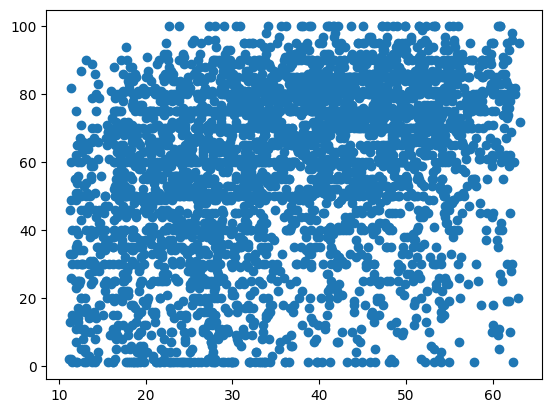
\includegraphics[width=0.9\linewidth, height=10cm, keepaspectratio]{images/data/__visualizations__/plt-scatter-dim1-rating-face-data.png}
    \caption{Scatter Plot (py-plt) output (face\_data.csv)}
\end{figure}
\end{minipage}
\hspace{0.2cm}
\vrule width 1pt
\hspace{0.5cm}
\begin{minipage}[t]{0.57\linewidth}
\begin{lstlisting}[
    language=Python,
    caption=Scatter Plot: py-plt: face\_data.csv
]
plt.scatter(df["dim1"], df["rating"])

plt.show()
\end{lstlisting}
\end{minipage}
\end{table}

\begin{table}[H]
\begin{minipage}[t]{0.35\linewidth}
\begin{figure}[H]
    \centering
    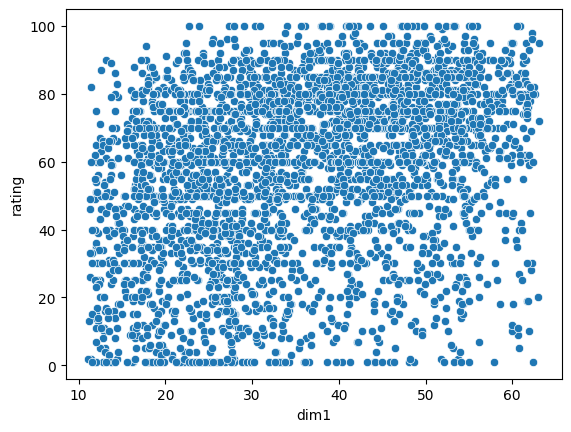
\includegraphics[width=0.9\linewidth, height=10cm, keepaspectratio]{images/data/__visualizations__/sns-scatter-dim1-rating-face-data.png}
    \caption{Scatter Plot (py-sns) output (face\_data.csv)}
\end{figure}
\end{minipage}
\hspace{0.2cm}
\vrule width 1pt
\hspace{0.5cm}
\begin{minipage}[t]{0.57\linewidth}
\begin{lstlisting}[
    language=Python,
    caption=Scatter Plot: py-sns: face\_data.csv
]
sns.scatterplot(df, x="dim1", y="rating")

plt.show()
\end{lstlisting}
\end{minipage}
\end{table}





\begin{enumerate}
    \item A scatter plot, also called a \textbf{scatterplot}, \textbf{scatter graph}\label{Visualizing Data/scatter graph}, \textbf{scatter chart}\label{Visualizing Data/scatter chart}, \textbf{scattergram}\label{Visualizing Data/scattergram}, or \textbf{scatter diagram}\label{Visualizing Data/scatter diagram}, is a type of plot or mathematical diagram using Cartesian coordinates to display values for typically two variables for a set of data. \hfill \cite{data/online/wiki/Scatter_plot}
    
    \item If the points are coded (color/shape/size), one additional variable can be displayed. \hfill \cite{data/online/wiki/Scatter_plot}
    
    \item The data are displayed as a collection of points, each having the value of one variable determining the position on the horizontal axis and the value of the other variable determining the position on the vertical axis. \hfill \cite{data/online/wiki/Scatter_plot}
\end{enumerate}






